Un conjunto horizontal masa--resorte, con \(m=2\,\mathrm{kg}\) y \(k=8\,\mathrm{N/m}\), viaja en un camión a \(1\,\mathrm{m/s}\).
El camión se detiene bruscamente y el extremo sujeto del resorte queda fijo. La masa se libera en ese instante, situada \(0.5\,\mathrm m\) por delante del equilibrio y con velocidad hacia delante \(1\,\mathrm{m/s}\) respecto al extremo fijo.
En el modelo ideal sin rozamiento, hallar la frecuencia y la amplitud de la oscilación posterior.

\Needspace{6.53cm}
\begin{center}
\begin{minipage}{\linewidth}
\centering
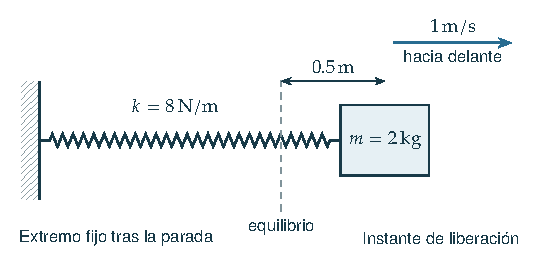
\includegraphics[width=10.22cm]{assets/M2-E0017-setup.pdf}\par
\smallskip{\small Configuración en el instante de liberación, con el extremo del muelle ya fijo.\par}
\end{minipage}
\end{center}
